\chapter{Introduction to the CLI}\label{introduction-to-the-cli}

\subsection{What is a CLI?}\label{what-is-a-cli}

\begin{itemize}
\tightlist
\item
  A ``Command-line Interface''
\item
  The interface you use to configure Cisco devices
\end{itemize}

A GUI is a ``Graphical User Interface''

\subsection{How do you connect to a Cisco
Device?}\label{how-do-you-connect-to-a-cisco-device}

\begin{itemize}
\tightlist
\item
  Console Port : When you first configure a device, you have to connect
  via the Console Port.
\end{itemize}

You can use a ``Rollover cable'' : DB9 serial connector to RJ45 OR a DB9
Serial to USB

\begin{figure}
\centering
\pandocbounded{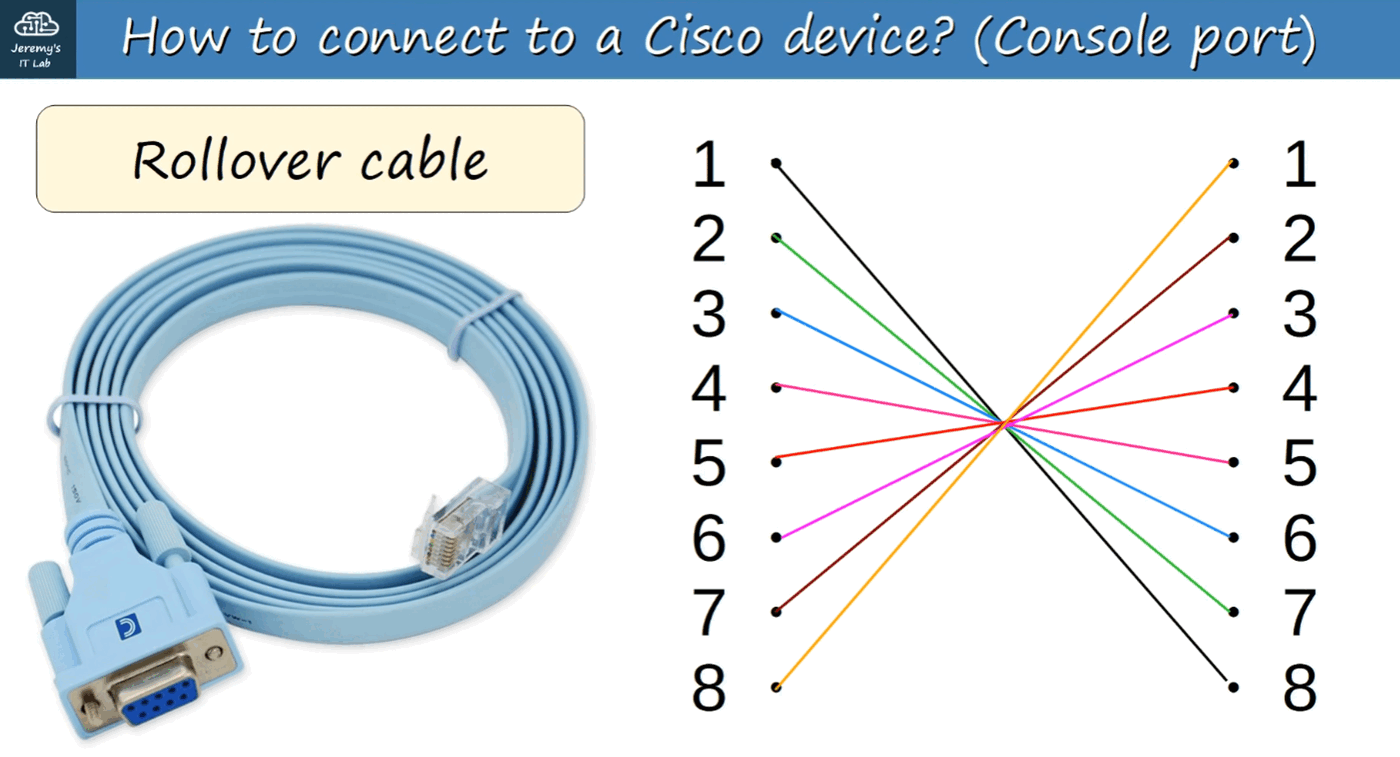
\includegraphics[keepaspectratio,alt={image}]{images/04-intro-to-cli/img-001.png}}
\end{figure}

\subsection{How do you actually access the
CLI?}\label{how-do-you-actually-access-the-cli}

\begin{itemize}
\tightlist
\item
  You need to use a TERMINAL EMULATOR (Example: PuTTy is a popular
  choice) and connect via ``Serial'' (default settings)
\end{itemize}

\subsection{Cisco Default Settings
are:}\label{cisco-default-settings-are}

Speed (baud) : 9600 bits/second Data bits: 8 data bits Stop bits: 1 stop
bit (sent after 8 data bits are sent) Parity: None Flow Control: None

When you first enter the CLI you will DEFAULT be in what is called `User
EXEC' mode.

\section{User Exec Mode}\label{user-exec-mode}

\begin{lstlisting}
(Hostname) >        // Prompt looks like THIS //
\end{lstlisting}

\begin{itemize}
\tightlist
\item
  User EXEC mode is very limited.
\item
  User can look at some things but can't make ANY changes to the
  configuration.
\item
  AKA `User Mode'
\end{itemize}

Using the `enable' command, in User EXEC mode, switches you to
`Privileged EXEC' mode.

\section{Privileged Exec Mode}\label{privileged-exec-mode}

\begin{itemize}
\tightlist
\item
  Provides complete access to view the device's configuration, restart
  the device, etc.
\item
  Cannot change the configuration, but can change the time on the
  device, save the configuration file, etc.
\end{itemize}

\begin{lstlisting}
(Hostname)#     // Prompt looks like THIS //
\end{lstlisting}

USE a Question Mark (?) to view the available commands in ANY mode.
Combining ? with a letter or partial command will list all the commands
with those letters.

\begin{figure}
\centering
\pandocbounded{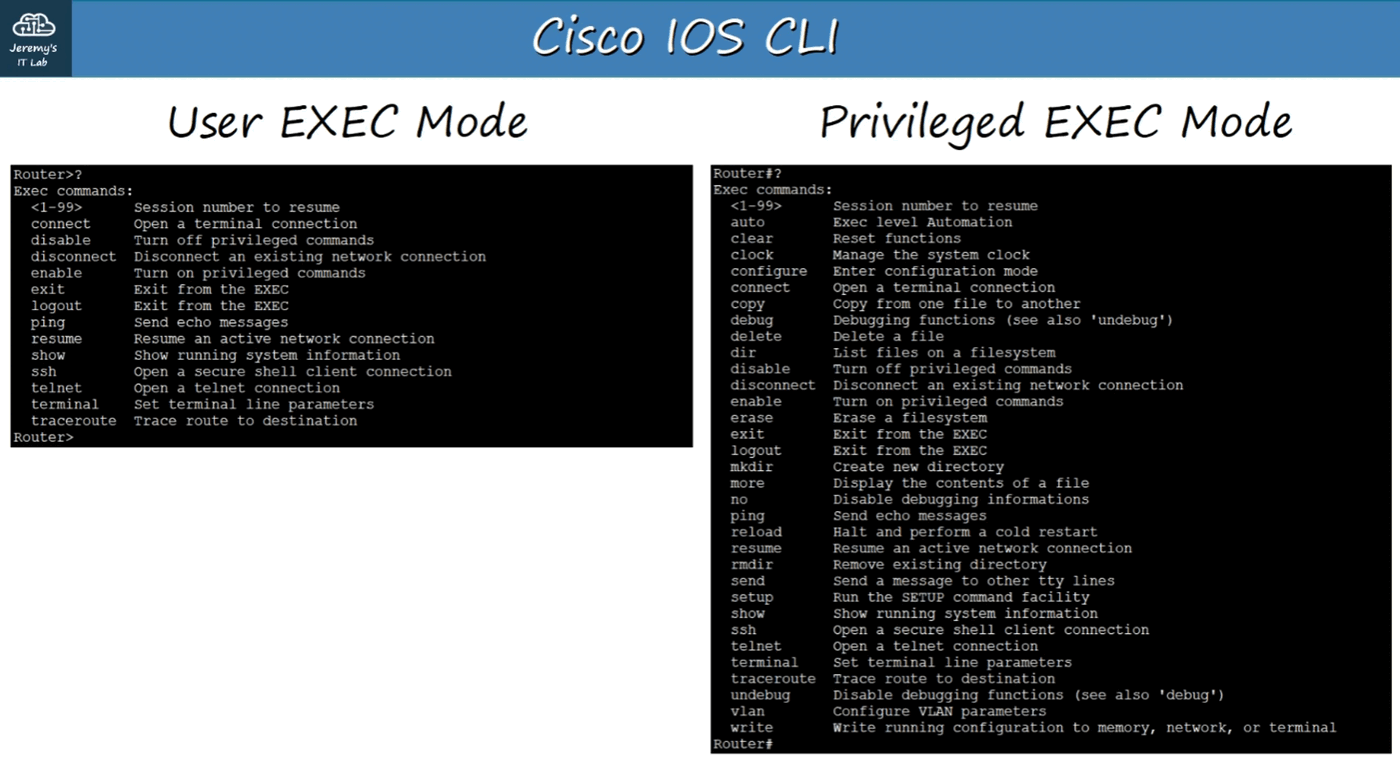
\includegraphics[keepaspectratio,alt={image}]{images/04-intro-to-cli/img-002.png}}
\end{figure}

USE the TAB key to complete partially entered commands IF the command
exists.

\subsection{GLOBAL CONFIGURATION MODE:}\label{global-configuration-mode}

To enter Global Configuration Mode, enter the command, within Privileged
EXEC mode

`configure terminal' (or `conf t')

Router\# configure terminal

Note the prompt change:

Router(config) \#

Type `exit' to drop back into `Privileged EXEC' mode.

\subsection{To Enable Password for User EXEC
mode:}\label{to-enable-password-for-user-exec-mode}

Router(config)\# enable password (password)

\begin{itemize}
\tightlist
\item
  Passwords ARE case-sensitive.
\end{itemize}

// This command encrypts plain-text passwords, visible in the config
files, using simple encryption.

Router(config)\# service password-encryption

If you enable `service password-encryption'

\begin{itemize}
\tightlist
\item
  Current passwords WILL be encrypted.
\item
  Future passwords WILL be encrypted.
\item
  The `enable secret' WILL NOT be effected.
\end{itemize}

If you disable `service password-encryption'

\begin{itemize}
\tightlist
\item
  Current passwords WILL NOT be decrypted.
\item
  Future passwords WILL NOT be encrypted.
\item
  The `enable secret' WILL NOT be effected.
\end{itemize}

// This command enables passwords for the Privileged EXEC mode.

Router(config)\# enable secret (password)

// enable secret will ALWAYS be encrypted (at level 5)

There are TWO separate configuration files kept on the device at once.

Running-config :

\begin{itemize}
\tightlist
\item
  The current, ACTIVE configuration file on the device. As you enter
  commands in the CLI, you edit the active configuration.
\end{itemize}

Startup-config :

\begin{itemize}
\tightlist
\item
  The configuration file that will be loaded upon RESTART of the device.
\end{itemize}

To see the configuration files, inside `Privileged EXEC' mode:

Router\# show running-config // for running config //

OR

Router\# show startup-config // for startup config //

To SAVE the Running configuration file, you can:

Router\# write Building configuration\ldots{} {[}OK{]}

Router\# write memory Building configuration\ldots{} {[}OK{]}

Router\# copy running-config startup-config

Destination filename {[}startup-config{]}?

Building configuration\ldots{} {[}OK{]}

To encrypt passwords:

Router\# conf t

Router(config)\# service password-encryption

This makes all current passwords \emph{encrypted}

Future passwords will ALSO be \emph{encrypted}

``Enable secret'' will not be effected (it's ALWAYS encrypted)

\begin{figure}
\centering
\pandocbounded{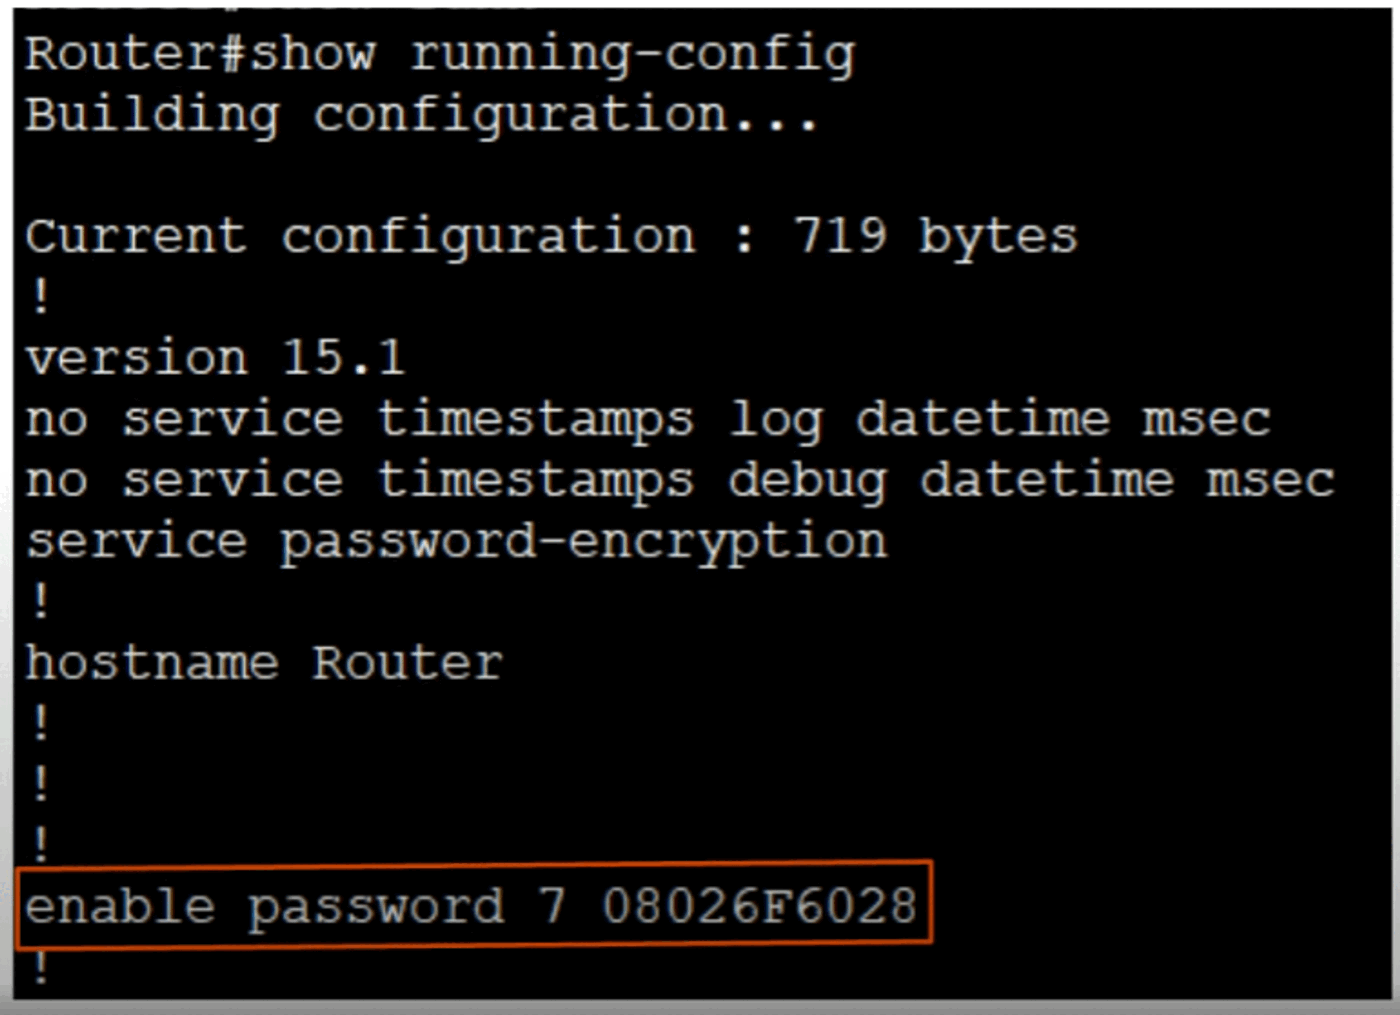
\includegraphics[keepaspectratio,alt={image}]{images/04-intro-to-cli/img-003.png}}
\end{figure}

Now you will see that the password is no longer in plaintext.

``7'' refers to the type of encryption used to encrypt the password. In
this case, ``7'' uses Cisco's proprietary encryption.

``7'' is fairly easy to crack since the encryption is weak.

For BETTER / STRONGER encryption, use ``enable secret''

\begin{figure}
\centering
\pandocbounded{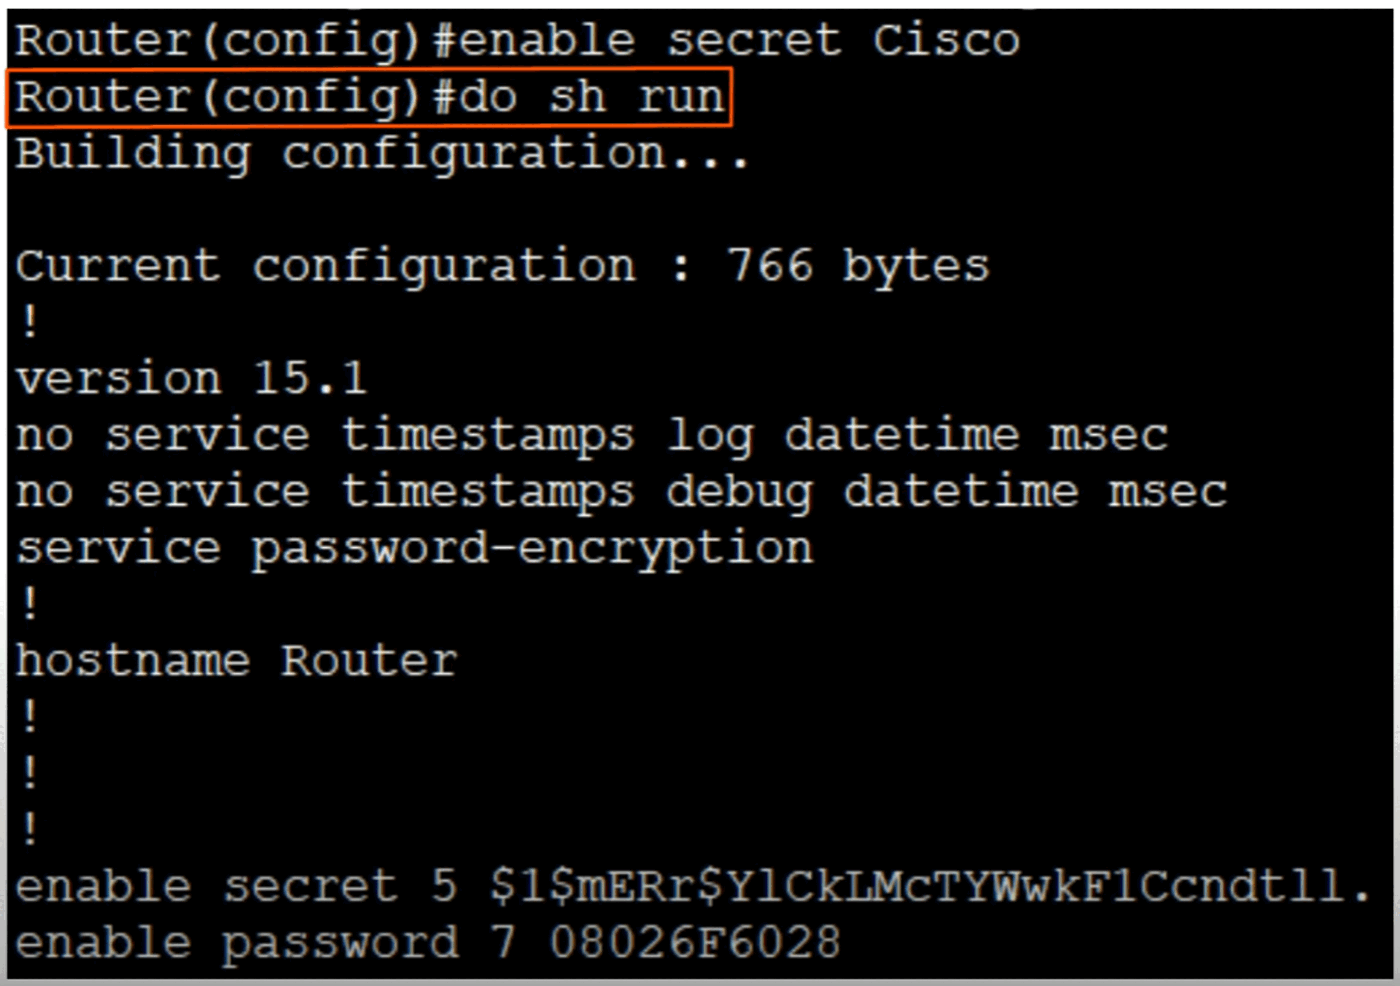
\includegraphics[keepaspectratio,alt={image}]{images/04-intro-to-cli/img-004.png}}
\end{figure}

``5'' refers to MD5 encryption.

Can still be cracked but it's much much stronger.

Once you use ``enable secret'' command, this will override ``enable
password''

To CANCEL or delete a command you entered, use the ``no'' keyword

\begin{figure}
\centering
\pandocbounded{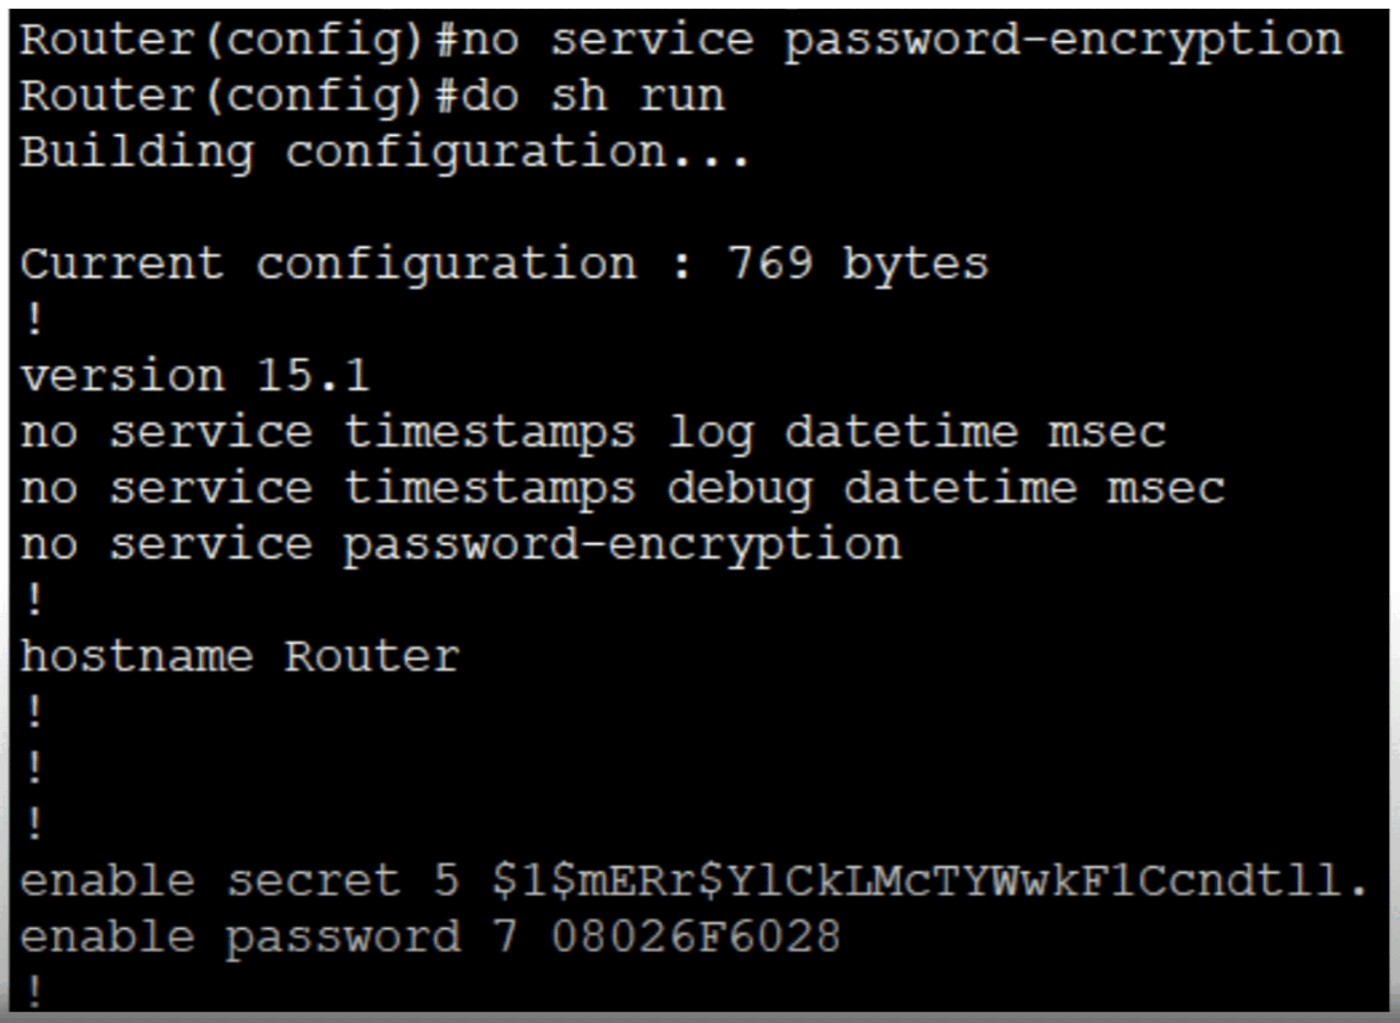
\includegraphics[keepaspectratio,alt={image}]{images/04-intro-to-cli/img-005.png}}
\end{figure}

In this instance, disabling ``service password-encryption'':

\begin{itemize}
\tightlist
\item
  current passwords will NOT be decrypted (unchanged)
\item
  future passwords will NOT be encrypted
\item
  the ``enable secret'' will not be effected
\end{itemize}

\begin{figure}
\centering
\pandocbounded{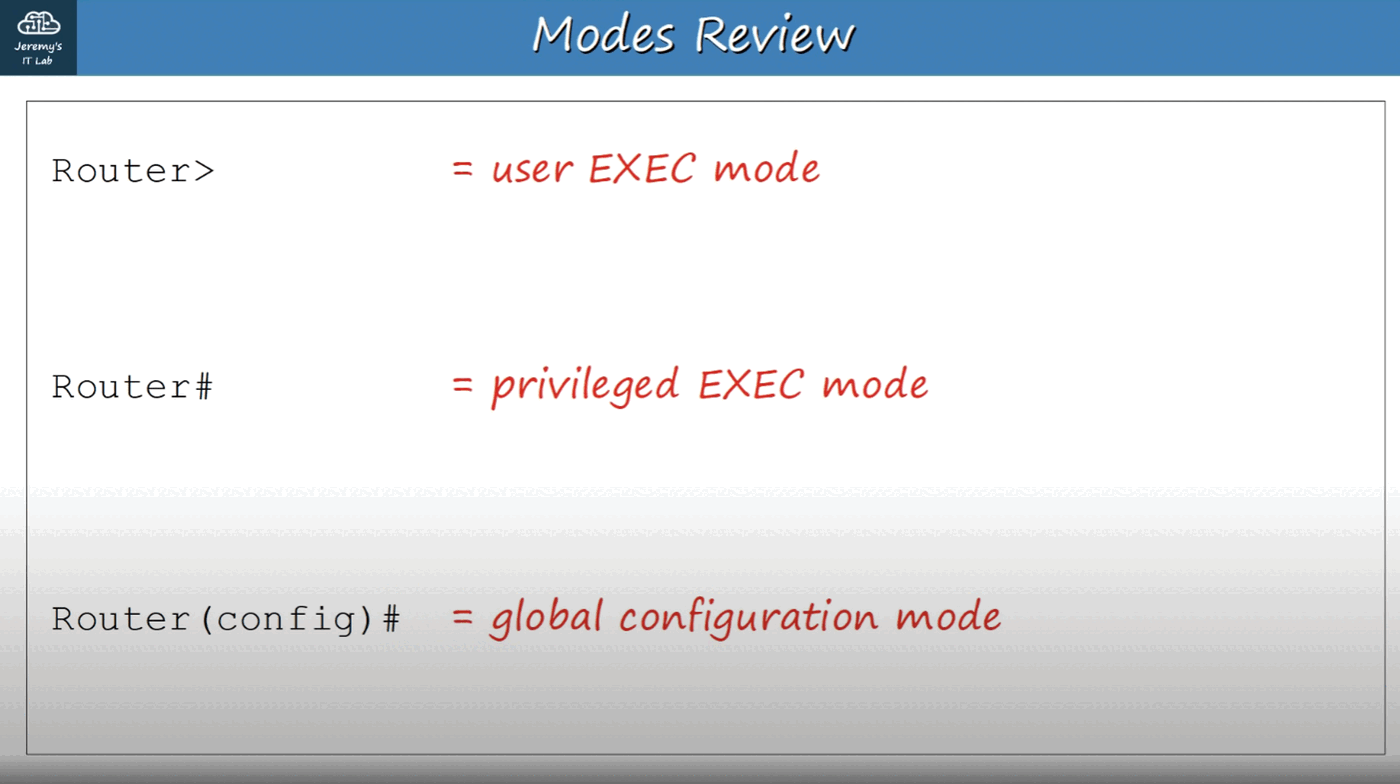
\includegraphics[keepaspectratio,alt={image}]{images/04-intro-to-cli/img-006.png}}
\end{figure}

\begin{figure}
\centering
\pandocbounded{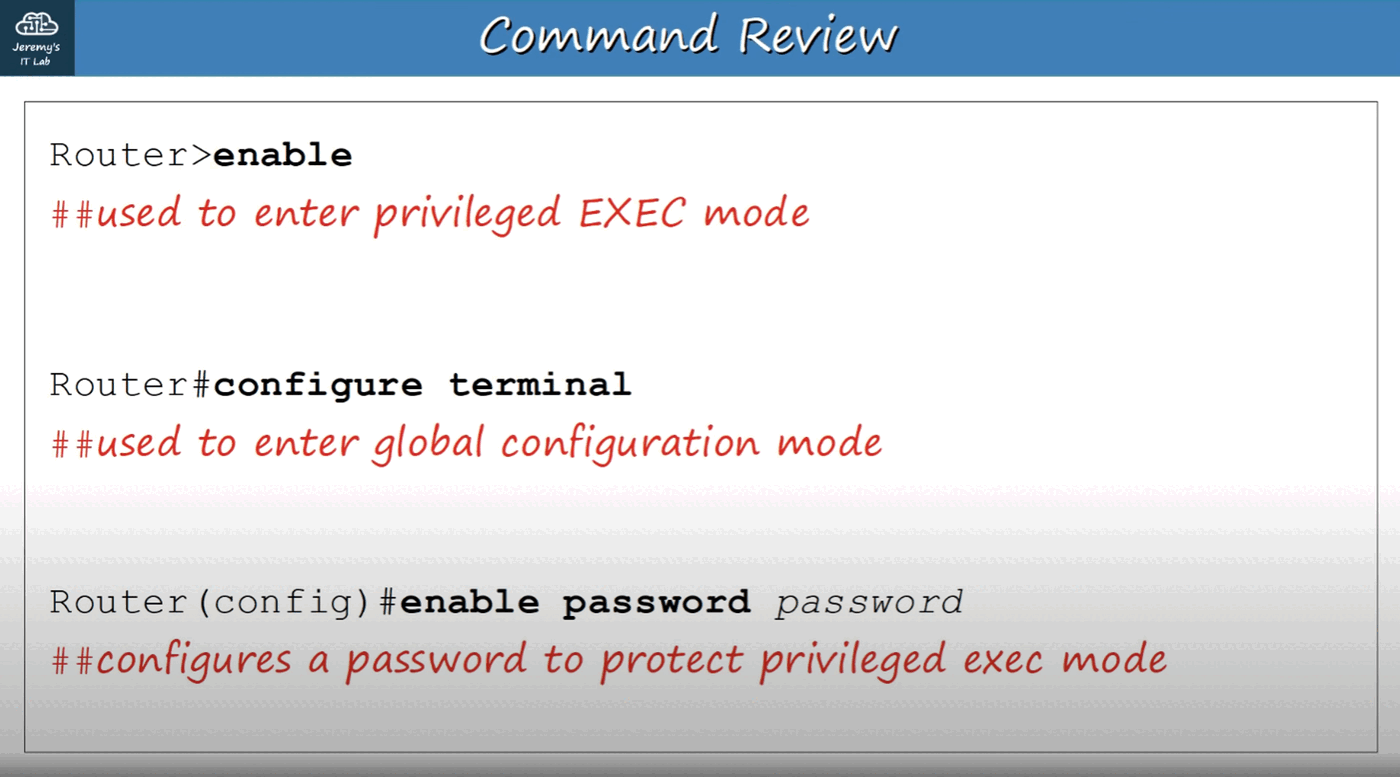
\includegraphics[keepaspectratio,alt={image}]{images/04-intro-to-cli/img-007.png}}
\end{figure}

\begin{figure}
\centering
\pandocbounded{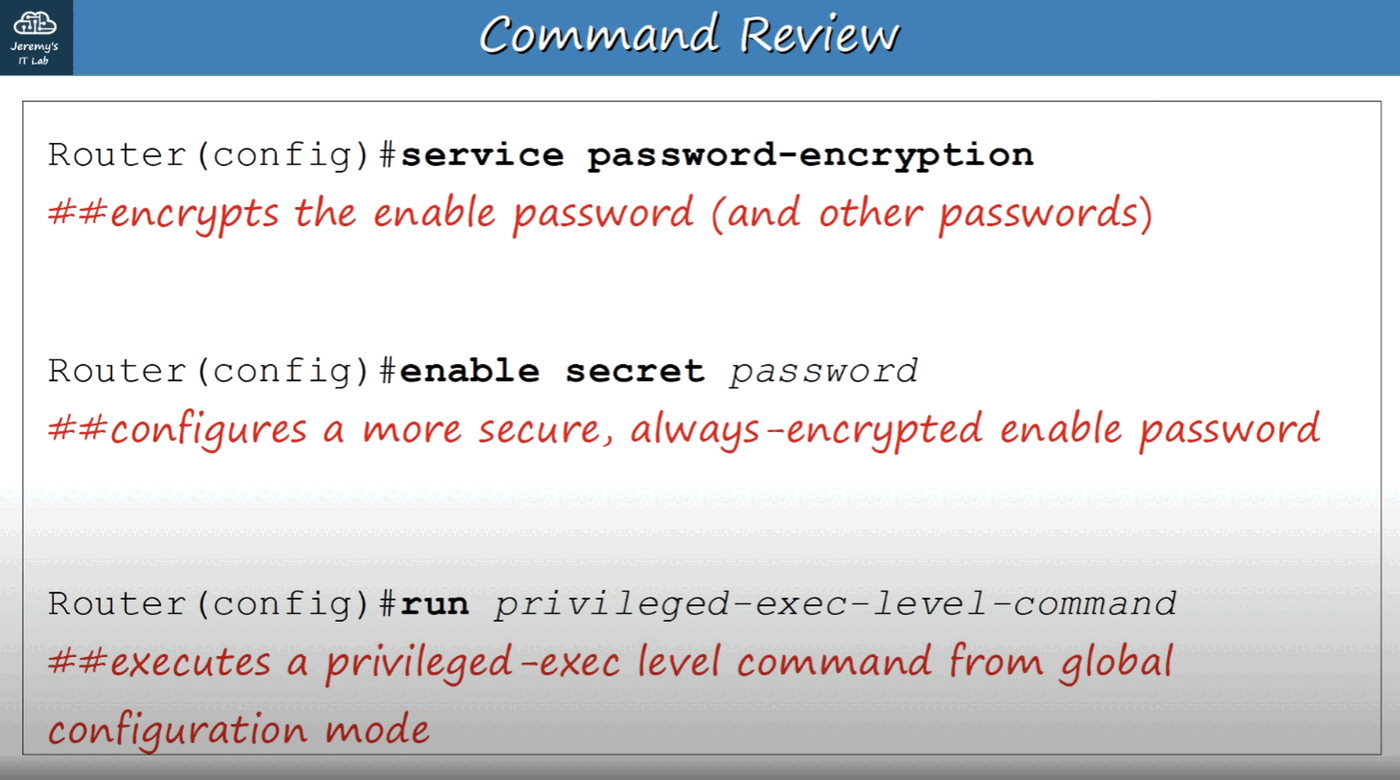
\includegraphics[keepaspectratio,alt={image}]{images/04-intro-to-cli/img-008.png}}
\end{figure}

\begin{figure}
\centering
\pandocbounded{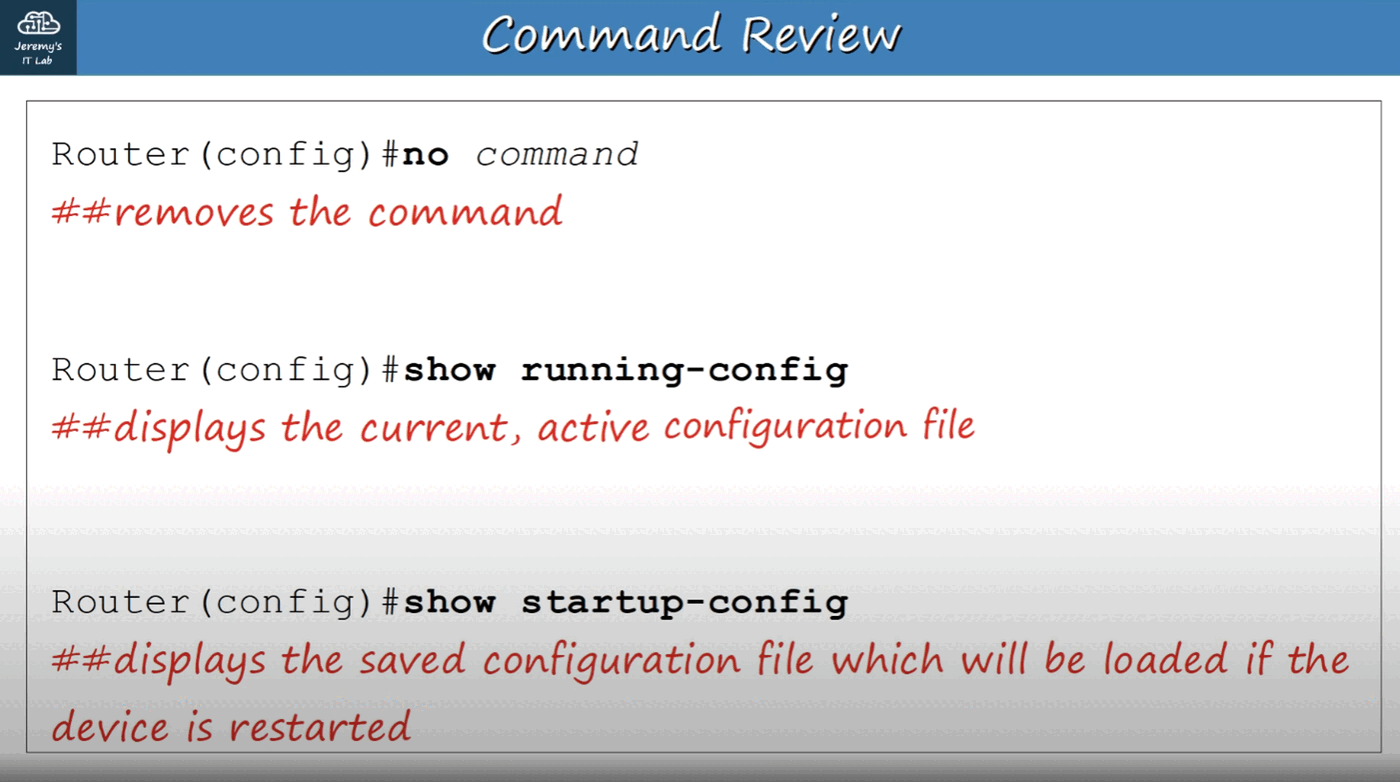
\includegraphics[keepaspectratio,alt={image}]{images/04-intro-to-cli/img-009.png}}
\end{figure}

\begin{figure}
\centering
\pandocbounded{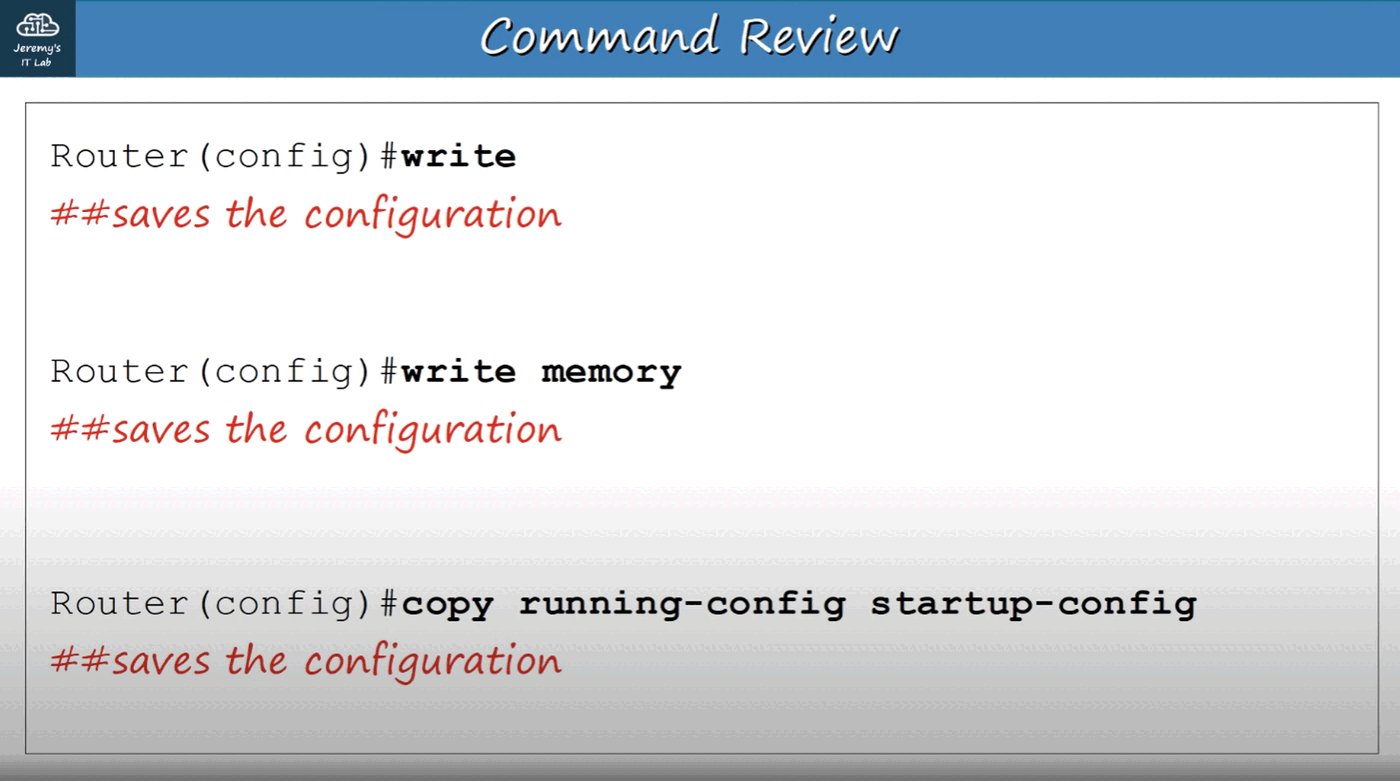
\includegraphics[keepaspectratio,alt={image}]{images/04-intro-to-cli/img-010.png}}
\end{figure}
